\documentclass[runningheads]{llncs}
\usepackage{graphicx}

\begin{document}

\title{Simplex vs. Montecarlo using parallel computing, a brief comparison.\thanks{Supported by Universidad Tecnológica de Pereira.}}

\author{Oscar Eduardo Bernal}

\authorrunning{O. Bernal}

\institute{Universidad Tecnológia de Pereira, Colombia
\email{}}

\maketitle        

\begin{abstract}
The Monte Carlo Method give us a process to solve big problems using randomness, by other side simplex is a method to solve linear optimization problems through an iterative process. Using HPC we can have an approach to parallel computing with a good amount of threads, but the Simplex method can't be easily parallelizable because in each iteration it depends of the previous state, while using Monte Carlo each step of the process is completely independent. Even so the question arises, is there really a difference between the Simplex method and the Monte Carlo method in a high-performance environment to solve linear optimization problems?

\keywords{HPC \and linear optimization \and Monte Carlo \and parallel computing \and Simplex}
\end{abstract}

\section{Introduction}
Is easy think that one algorithm is better than other, especially when we are working with parallel computing, but to give a conclusion like this, is needed to have a good comprehension of the subject, the algorithm and made a experimentation process, where we can check, using real information, the given hypothesis.

\subsection{Linear Optimization}
The Linear Optimization, also known as Linear Programming, is in the field of Mathematical optimization, a method to resolve problems where the target is achieve the best outcome subject to some requirements represented by linear inequality constraints.
Linear programming can be applied to various fields of study. It is widely used in mathematics, in business, economics, and for some engineering problems.

\subsection{Simplex Method}
The simplex method (or simplex algorithm) is a popular algorithm for linear programming, it uses the constraints as edges of a n-dimensional geometric object called a polytope (where n in the number of variables of the optimization problem), is an pivoting algorithm that do a iterative path over the vertices of the polytope to find the optimal solution.

\subsection{Monte Carlo Method}
Monte Carlo Method is a non deterministic computerized mathematical technique that allows to get an approximation to the solution of complex mathematical problems, Its fundamental idea is use randomness to solve the problems generating and evaluating points. 

\subsection{Parallel computing}
Parallel computing is a computational technique in which many instructions are executed simultaneously, one of his main principles is that large problems can often be divided into smaller problems and solved individually.

\subsection{Hypothesis}
Taking the capacity of Monte Carlo method to solve a large different kinds of problem, to solve linear optimization and mixing with the parallel computing technique appear the main hypothesis of this paper:

\textit{Monte Carlo method is better than Simplex method to solve linear optimization problems with large number of variables.}

\section{Implementation}
To test the validation of the given hypothesis, the two methods (Simplex and Monte Carlo) have been developed, the Simplex in a basic sequential way, and the Monte Carlo method in a concurrent way.

\subsection{Sequential Simplex Method}
The simplex method takes the constraints and the objective function of the linear optimization problem and creates a matrix of nxm dimensions, where n is the number of variables and m the number of constraints, over this matrix the algorithm starts to iterate changing the values of some rows and columns until arrives to the optimal solution.
This algorithm have a quadratic complexity order O(n\textsuperscript{2}) in the worst case, and a lineal complexity order O(n) in its best case.

\subsection{Parallel Monte Carlo Method}
The concurrent implementation of the Monte Carlo Method starts whit a fixed amount of threads for each block, for this case 1024, and a fixed amount of blocks per grid, that also is 1024, for the logical distribution of the threads and blocks, that can be given by the size of the grid/block in terms of \textit x, \textit y and \textit z, was used a lineal distribution (\textit{x,1,1}), this aiming to make more clear and intuitive the index generation for the resultant vector; Anyway with little modifications can be extended to a full tri-dimensional distribution.

\paragraph{}
The kernel of this implementation generate an fixed amount of random numbers under the constraints and validating the objective function to find an individual optimal solution, all the solutions obtained by each thread are write in the thread's correspondent index of the resultant vector, after this process finished, in the vector is found the best solution.
By this way the number generation have a lineal complexity order O(n), and the find of the best solution too.

\section{Results}
After the execution of the implemented methods for linear optimization problems with a different number of variables and constraints, the execution times shows a unlooked-for results, although the behavior of the algorithms corresponds to the determinated complexity, the scale of the measures is completely unexpected. 
For this reason, the importance of experimentation is remarkable.

\begin{figure}
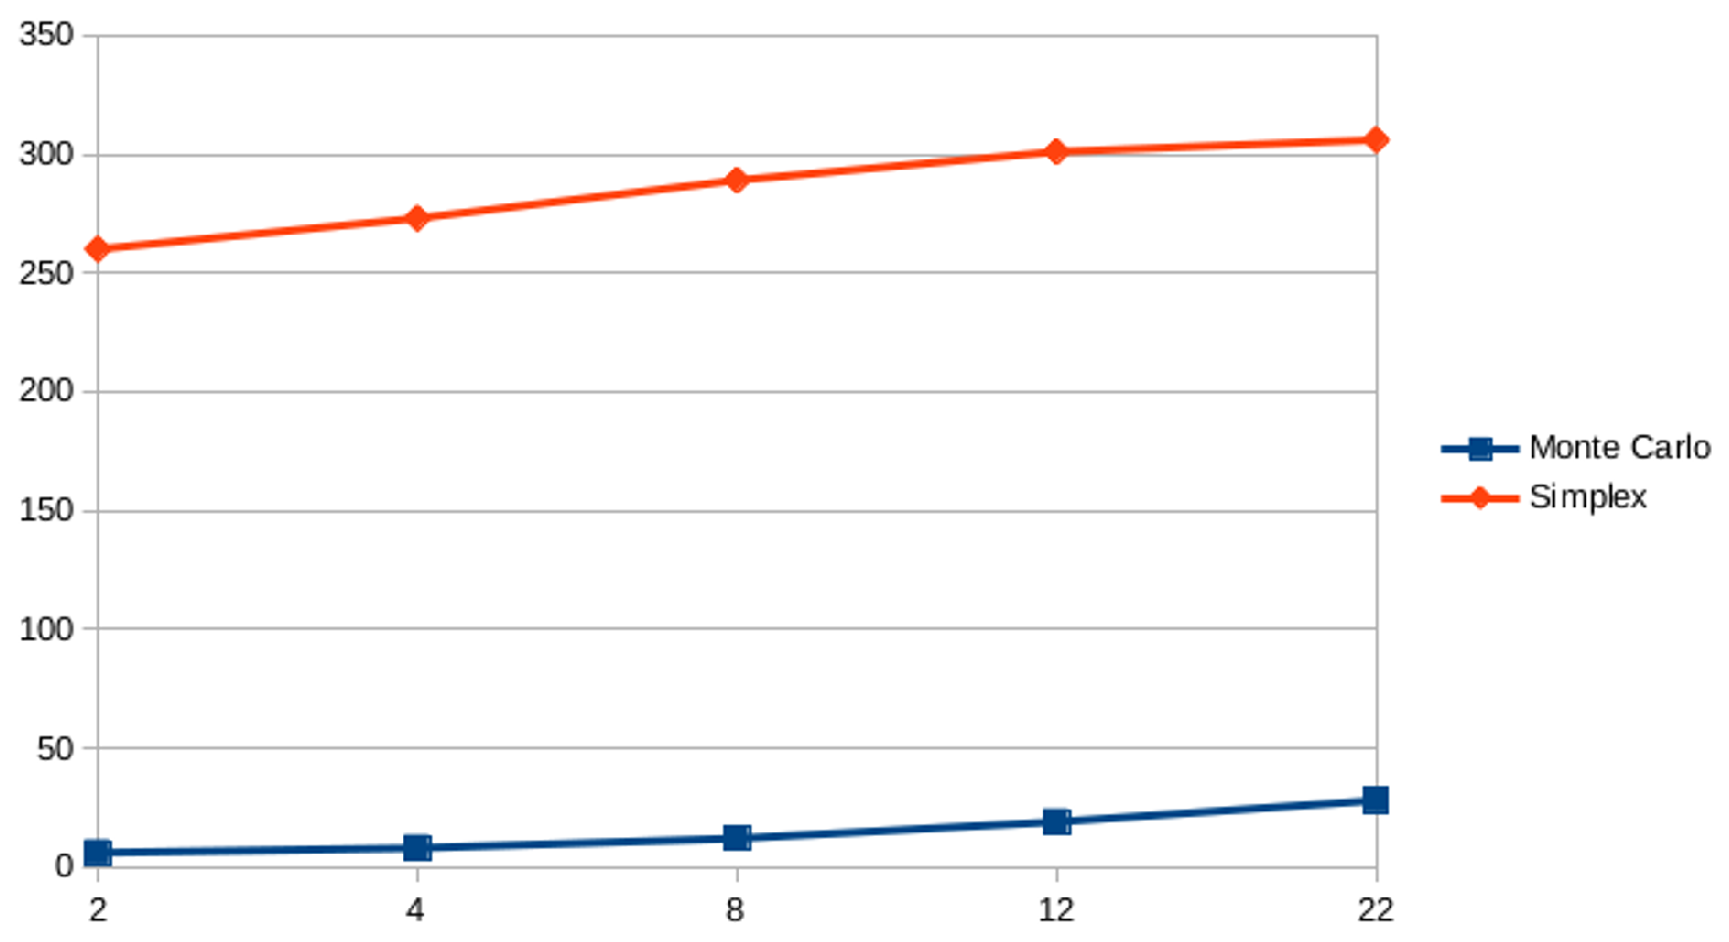
\includegraphics[width=\textwidth]{fig1.eps}
\caption{Execution time in milliseconds for each algorithm} \label{fig1}
\end{figure}

\paragraph{}
By this way we have the Simplex method with a quadratic complexity order O(n\textsuperscript{2}) in the worst case, but here is where the core of behavior of the results, the worst case is an stranger case, the common case of the majority of the linear optimization problems are solved in a a lineal complexity order O(n) by the Simplex method, causing so the Monte Carlo method take superior execution times that the sequential Simplex.

\paragraph{}
In addition was observed, during the data collection, that linear optimization problems with a large number of variables were hardly found, the largest problem easily founded was of 8 variables, all other problems were artificially constructed to test the behavior of the methods. The largest problem tested was 22 variables and 23 restrictions.

\paragraph{}
This means that even if Monte Carlo have better execution times with a gigantic amount of variables, it is useless because the common linear optimization problems have a low number of variables.

\paragraph{}
The Monte Carlo method, unlike the Simplex method, finds an approximate values really close to the expected response ($Error=1/\sqrt{n}$ , with n equal to the total amount of threads times the number of solutions generated in each thread), but not always the exact value, and in this an important advantage for the Simplex Method, because it get the better answer (if the problem has a unique solution).Besides in the cases where the problem don't have an unique solution, Monte Carlo method finds a feasible solution, instead of being blocked as the simplex method.

\paragraph{}
For nonlinear optimization problems the Monte Carlo method can be adapted with few changes and conserving its properties, while the simplex method becomes useless and requires different methods that change depending on the kind of problem.

\section{Conclusions}

\paragraph{}
Not always parallel is better, it is easy to think that by using a parallel alternative for the solution of a problem we can obtain better results, but this always depends on the nature of the problem and it is necessary to have a correct analysis to determine if the implementation of a parallel method is the best option.

\paragraph{}
The complexity order of an algorithm is a great help to know the possible performance of it is, but also should keep in mind the common behavior of the algorithm, because there is a possibility that the common case is not the worst case.

\paragraph{}
In every process of experimentation it is important to have clearly defined the hypothesis and do a good analysis of the problem, but also pay attention to the results and the experience, because the result will not always be as expected and it is important to determine the explanation of these results.

\paragraph{}
High performance computing is a technology that offers many possibilities, but as any technological tool must be used with responsibility. The capacity of the developments made using HPC techniques will depend on the formulation and implementation of the correct kind of algorithms. 

\paragraph{}
The Monte Carlo method allows to solve a whole range of different problems, while the simplex method specializes in a single class of problems but is very good in it. By this way we can concluded that a general solution is not always the best alternative, sometimes it is better to have solutions optimized to the requirements of the problem, and for this reason is important to do a correct analysis of the problem.

%
% ---- Bibliography ----
%
% BibTeX users should specify bibliography style 'splncs04'.
% References will then be sorted and formatted in the correct style.
%
% \bibliographystyle{splncs04}
% \bibliography{mybibliography}
%
\begin{thebibliography}{8}

\bibitem{ref_url1}
Monte Carlo Simulation: What Is It and How Does It Work? - Palisade, \url{http://www.palisade.com/risk/monte\_carlo\_simulation.asp}. Last accessed
Jun 2018

\bibitem{ref_url1}
A Gentle Introduction to Algorithm Complexity Analysis, \url{https://discrete.gr/complexity/}. Last accessed
Jun 2018

\bibitem{ref_article1}
Roughgarden, T. (2014). CS264: Beyond Worst-Case Analysis Lecture\# 15: Smoothed Complexity and Pseudopolynomial-Time Algorithms. Retrieved from \url{https://pdfs.semanticscholar.org/395c/5adcd11e95b8ec174ec359be54452fdb27a2.pdf}

\bibitem{ref_article1}
Smale, S. Mathematical Programming (1983) 27: 241. \doi{10.1007/BF02591902}

\bibitem{ref_article1}
Borgwardt, K.H. Zeitschrift für Operations Research (1982) 26: 157. \doi{10.1007/BF01917108}

\bibitem{ref_article1}
Lovász, L. The Mathematical Intelligencer (1980) 2: 141. \doi{10.1007/BF03023055}

\bibitem{ref_book1}
Bertsimas, D., \& Tsitsiklis, J. N. (1997). Introduction to linear optimization (Vol. 6, pp. 479-530). Belmont, MA: Athena Scientific.

\bibitem{ref_book1}
Doucet A., de Freitas N., Gordon N. (2001) An Introduction to Sequential Monte Carlo Methods. In: Doucet A., de Freitas N., Gordon N. (eds) Sequential Monte Carlo Methods in Practice. Statistics for Engineering and Information Science. Springer, New York, NY
\end{thebibliography}

\end{document}
